\subsection{Distribution of the variables inside \gls{sr}}

The following figures (\autoref{fig:distributions1} and \autoref{fig:distributions2}) show the distributions of some variables
of interest inside \gls{sr}.

\captionsetup[subfigure]{justification=centering}
\begin{figure}[htb!]
    \centering
    \begin{subfigure}{0.45\textwidth}
        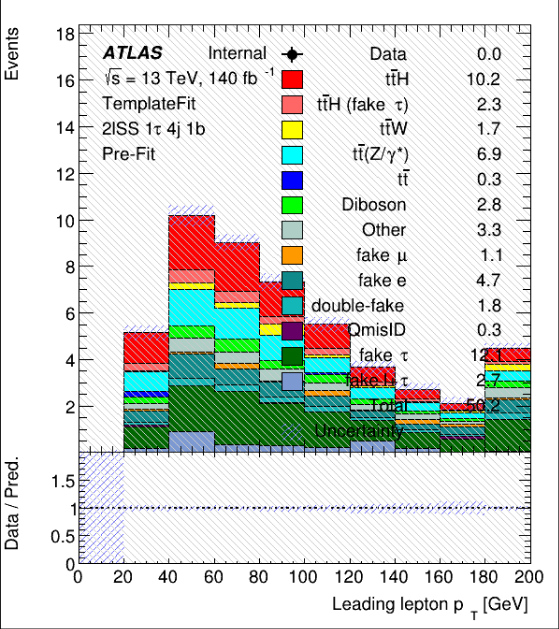
\includegraphics[width=\linewidth]{figures/plots/histograms/lep_pt_0.png}
        \caption{Distribution of the transverse momentum of the leading lepton.}
        \label{fig:lep_pt_0}
    \end{subfigure}\hfill%
    \begin{subfigure}{0.45\textwidth}
        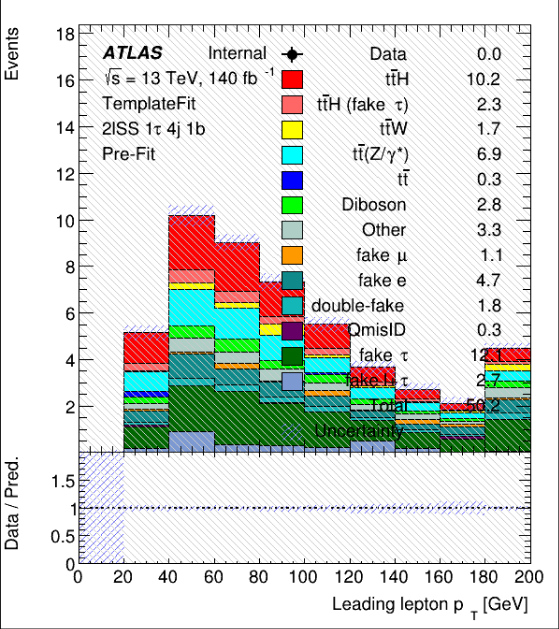
\includegraphics[width=\linewidth]{figures/plots/histograms/lep_pt_1.png}
        \caption{Distribution of the transverse momentum of the subleading lepton.}
        \label{fig:lep_pt_1}
    \end{subfigure}

    \vspace{0.5cm}

    \begin{subfigure}{0.45\textwidth}
        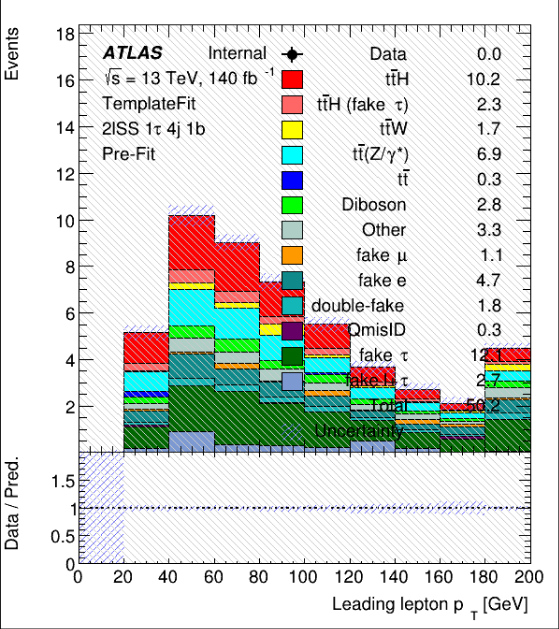
\includegraphics[width=\linewidth]{figures/plots/histograms/lep_Eta_0.png}
        \caption{Distribution of the pseudorapidity of the leading lepton.}
        \label{fig:lep_Eta_0}
    \end{subfigure}\hfill%
    \begin{subfigure}{0.45\textwidth}
        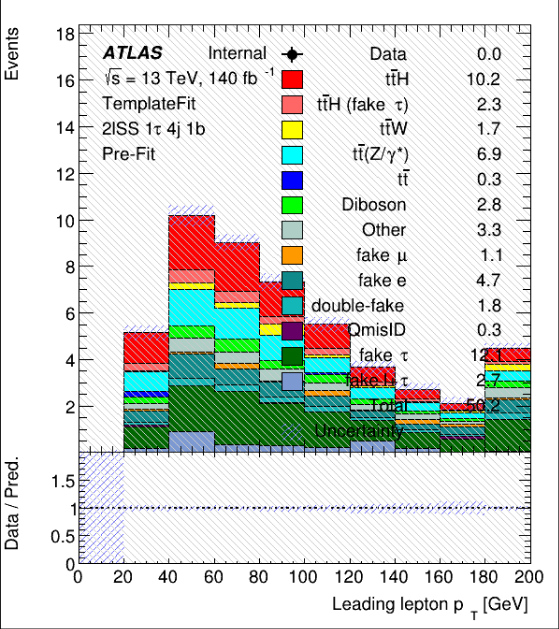
\includegraphics[width=\linewidth]{figures/plots/histograms/lep_Eta_1.png}
        \caption{Distribution of the pseudorapidity of the subleading lepton.}
        \label{fig:lep_Eta_1}
    \end{subfigure}
    \caption{Distributions of the variables inside \gls{sr} (part 1)}
    \label{fig:distributions1}
\end{figure}

\newpage

\begin{figure}[htb!]
    \centering
    \begin{subfigure}{0.45\textwidth}
        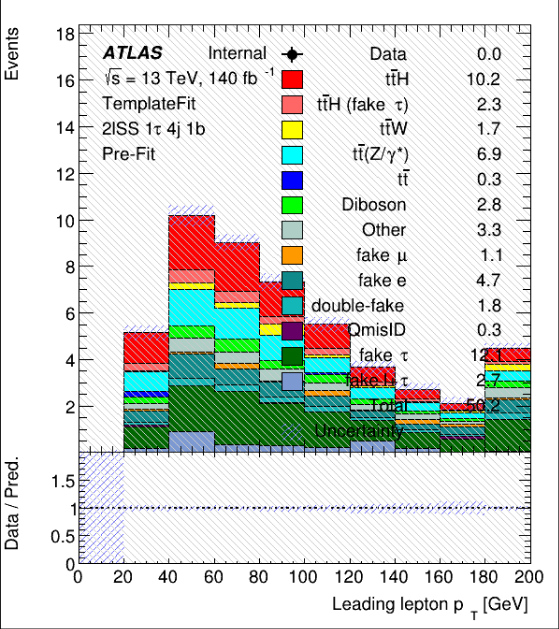
\includegraphics[width=\linewidth]{figures/plots/histograms/lep_Phi_0.png}
        \caption{Distribution of the azimuthal angle of the leading lepton.}
        \label{fig:lep_Phi_0}
    \end{subfigure}\hfill%
    \begin{subfigure}{0.45\textwidth}
        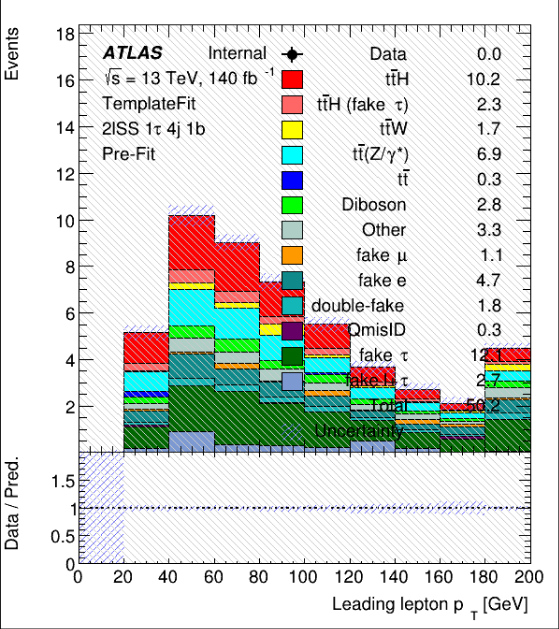
\includegraphics[width=\linewidth]{figures/plots/histograms/lep_Phi_1.png}
        \caption{Distribution of the azimuthal angle of the subleading lepton.}
        \label{fig:lep_Phi_1}
    \end{subfigure}

    \vspace{0.5cm}

    \begin{subfigure}{0.45\textwidth}
        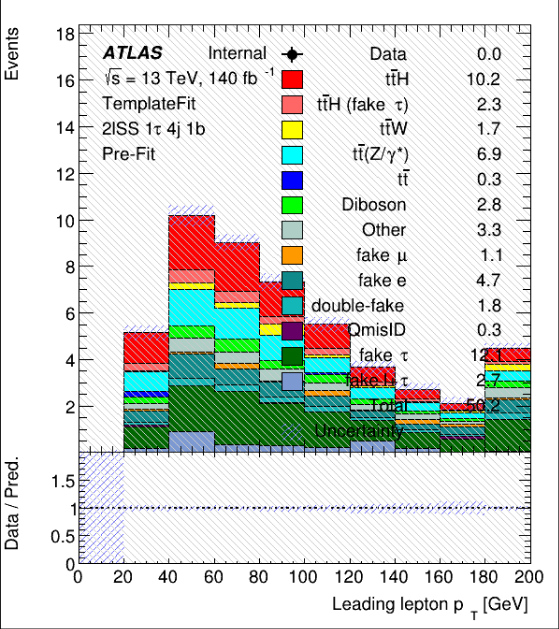
\includegraphics[width=\linewidth]{figures/plots/histograms/njets.png}
        \caption{Distribution of the number of jets.}
        \label{fig:njets}
    \end{subfigure}\hfill%
    \begin{subfigure}{0.45\textwidth}
        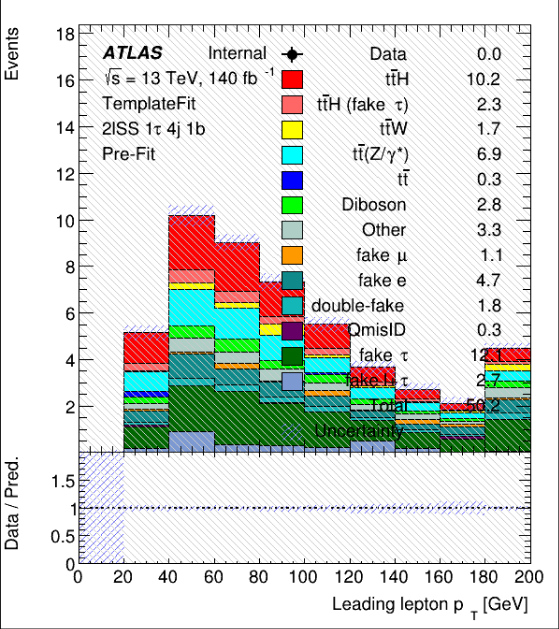
\includegraphics[width=\linewidth]{figures/plots/histograms/nbjets.png}
        \caption{Distribution of the number of $b$-jets.}
        \label{fig:nbjets}
    \end{subfigure}
    \caption{Distributions of the variables inside \gls{sr} (part 2)}
    \label{fig:distributions2}
\end{figure}

\begin{minipage}{0.45\textwidth}
    \centering
    \begin{tabular}{c|c|c|c|c}
        $t\bar{t}H$ & \textbf{v6} & \textbf{v8} &      &       \\
        \hline
        Weighted    & 1000        & 500         & -500 & -50\% \\
        Raw         & 1000        & 500         & -500 & -50\% \\
        \hline
    \end{tabular}
    \captionof{table}{Number of ttH events in the SR for v6 and v8.}
    \label{tab:ttH_event_numbers1}
\end{minipage}\hfill%
\begin{minipage}{0.45\textwidth}
    \centering
    \begin{tabular}{c|c|c|c|c}
        \gls{sr} & \textbf{v6} & \textbf{v8} &      &       \\
        \hline
        Weighted & 1000        & 500         & -500 & -50\% \\
        Raw      & 1000        & 500         & -500 & -50\% \\
        \hline
    \end{tabular}
    \captionof{table}{Number of all the events in the SR for v6 and v8.}
    \label{tab:ttH_event_numbers2}
\end{minipage}
